% Options for packages loaded elsewhere
\PassOptionsToPackage{unicode}{hyperref}
\PassOptionsToPackage{hyphens}{url}
%
\documentclass[
  12pt,a4paper,lualatex,ja=standard]{bxjsarticle}
\usepackage{lmodern}
\usepackage{amsmath}
\usepackage{ifxetex,ifluatex}
\ifnum 0\ifxetex 1\fi\ifluatex 1\fi=0 % if pdftex
  \usepackage[T1]{fontenc}
  \usepackage[utf8]{inputenc}
  \usepackage{textcomp} % provide euro and other symbols
  \usepackage{amssymb}
\else % if luatex or xetex
  \usepackage{unicode-math}
  \defaultfontfeatures{Scale=MatchLowercase}
  \defaultfontfeatures[\rmfamily]{Ligatures=TeX,Scale=1}
\fi
% Use upquote if available, for straight quotes in verbatim environments
\IfFileExists{upquote.sty}{\usepackage{upquote}}{}
\IfFileExists{microtype.sty}{% use microtype if available
  \usepackage[]{microtype}
  \UseMicrotypeSet[protrusion]{basicmath} % disable protrusion for tt fonts
}{}
\makeatletter
\@ifundefined{KOMAClassName}{% if non-KOMA class
  \IfFileExists{parskip.sty}{%
    \usepackage{parskip}
  }{% else
    \setlength{\parindent}{0pt}
    \setlength{\parskip}{6pt plus 2pt minus 1pt}}
}{% if KOMA class
  \KOMAoptions{parskip=half}}
\makeatother
\usepackage{xcolor}
\IfFileExists{xurl.sty}{\usepackage{xurl}}{} % add URL line breaks if available
\IfFileExists{bookmark.sty}{\usepackage{bookmark}}{\usepackage{hyperref}}
\hypersetup{
  hidelinks,
  pdfcreator={LaTeX via pandoc}}
\urlstyle{same} % disable monospaced font for URLs
\usepackage{graphicx}
\makeatletter
\def\maxwidth{\ifdim\Gin@nat@width>\linewidth\linewidth\else\Gin@nat@width\fi}
\def\maxheight{\ifdim\Gin@nat@height>\textheight\textheight\else\Gin@nat@height\fi}
\makeatother
% Scale images if necessary, so that they will not overflow the page
% margins by default, and it is still possible to overwrite the defaults
% using explicit options in \includegraphics[width, height, ...]{}
\setkeys{Gin}{width=\maxwidth,height=\maxheight,keepaspectratio}
% Set default figure placement to htbp
\makeatletter
\def\fps@figure{htbp}
\makeatother
\setlength{\emergencystretch}{3em} % prevent overfull lines
\providecommand{\tightlist}{%
  \setlength{\itemsep}{0pt}\setlength{\parskip}{0pt}}
\setcounter{secnumdepth}{5}
\usepackage{indentfirst}
\parindent = 1em
\usepackage{dcolumn}
\newcolumntype{.}{D{.}{.}{-1}}
\usepackage{caption}
\captionsetup[table]{name=表}
\captionsetup[figure]{name=図}
\usepackage{hyperref}
\pagestyle{empty}
\usepackage{multicol}
\usepackage{ascmac}
\setpagelayout*{top=10truemm,bottom=30truemm,left=10truemm,right=10truemm}
\usepackage{tikz}
\usetikzlibrary{arrows.meta,decorations,decorations.pathreplacing}
\usepackage{tabstackengine}
\usepackage{xcolor}
\usepackage{rotating}
\usepackage{txfonts}
\usepackage{fancybox}
\usepackage{dashbox}
\usepackage{tcolorbox}
\tcbuselibrary{theorems,skins}
\usepackage{siunitx}
\usepackage{framed}
\usepackage{enumerate}
\usepackage{lastpage}
\usepackage{pxrubrica}
\ifluatex
  \usepackage{selnolig}  % disable illegal ligatures
\fi

\author{}
\date{\vspace{-2.5em}}

\begin{document}

\renewcommand{\thefootnote}{}
\newcounter{kaunta}
\renewcommand{\thekaunta}{\arabic{kaunta}}
\newcommand{\kaunta}{\refstepcounter{kaunta}%
\thekaunta}
\def\question{\noindent\fbox{\large\makebox[1em]{\text{\kaunta}}} \hspace{1pt}}
\newcounter{skaunta}
\renewcommand{\theskaunta}{\arabic{skaunta}}
\newcommand{\skaunta}{\refstepcounter{skaunta}%
\theskaunta}
\def\squestion{(\text{\skaunta})\hspace{2.5pt}}
\newcommand{\maru}[1]{\raise0.2ex\hbox{\textcircled{\scriptsize{#1}}}}
\newcommand{\jsim}{\mathrel{\text{∽}}}
\newcommand{\jpara}{/\!/}

\newcounter{kcounter}
\setcounter{kcounter}{0}
\newcommand{\kana}{\refstepcounter{kcounter}\ifthenelse{\value{kcounter}=1}{ア}{\ifthenelse{\value{kcounter}=2}{イ}{\ifthenelse{\value{kcounter}=3}{ウ}{\ifthenelse{\value{kcounter}=4}{エ}{\ifthenelse{\value{kcounter}=5}{オ} {\ifthenelse{\value{kcounter}=6}{カ}{\ifthenelse{\value{kcounter}=7}{キ}{\ifthenelse{\value{kcounter}=8}{ク}{\ifthenelse{\value{kcounter}=9}{ケ}{\ifthenelse{\value{kcounter}=10}{コ}{\ifthenelse{\value{kcounter}=11}{サ}{\ifthenelse{\value{kcounter}=12}{シ}{\ifthenelse{\value{kcounter}=13}{ス}{\ifthenelse{\value{kcounter}=14}{セ}{\ifthenelse{\value{kcounter}=15}{ソ}{\ifthenelse{\value{kcounter}=16}{タ}{\ifthenelse{\value{kcounter}=17}{チ}{\ifthenelse{\value{kcounter}=18}{ツ}{\ifthenelse{\value{kcounter}=19}{テ}{\ifthenelse{\value{kcounter}=20}{ト}{\ifthenelse{\value{kcounter}=21}{ナ}{\ifthenelse{\value{kcounter}=22}{二}{\ifthenelse{\value{kcounter}=23}{ヌ}{\ifthenelse{\value{kcounter}=24}{ネ}{\ifthenelse{\value{kcounter}=25}{ノ}{\ifthenelse{\value{kcounter}=26}{ハ}{\ifthenelse{\value{kcounter}=27}{ヒ}{\ifthenelse{\value{kcounter}=28}{フ}{\ifthenelse{\value{kcounter}=29}{ヘ}{\ifthenelse{\value{kcounter}=30}{ホ}{\ifthenelse{\value{kcounter}=31}{マ}{\ifthenelse{\value{kcounter}=32}{ミ}{\ifthenelse{\value{kcounter}=33}{ム}{\ifthenelse{\value{kcounter}=34}{メ}{\ifthenelse{\value{kcounter}=35}{モ}{\ifthenelse{\value{kcounter}=36}{ヤ}{\ifthenelse{\value{kcounter}=37}{ユ}{\ifthenelse{\value{kcounter}=38}{ヨ}{\ifthenelse{\value{kcounter}=39}{ラ}{\ifthenelse{\value{kcounter}=40}{リ}{\ifthenelse{\value{kcounter}=41}{ル}{\ifthenelse{\value{kcounter}=42}{レ}{\ifthenelse{\value{kcounter}=43}{ロ}{\ifthenelse{\value{kcounter}=44}{ワ}{・}}}}}}}}}}}}}}}}}}}}}}}}}}}}}}}}}}}}}}}}}}}}}

\newcommand{\kuran}[1]{\framebox[1.5cm][c]{\maru{#1}}}

\newcommand{\haiten}[1]{%
\begin{flushright}%
\footnotesize{<#1>}%
\end{flushright}%
}

\newgeometry{top=10truemm,bottom=10truemm,left=20truemm,right=20truemm}

\thispagestyle{empty}
\begin{center}
\phantom{empty}

\vspace{60truemm}

\hspace{4em} {\HUGE\gtfamily\bfseries \ruby[g]{数}{すう}\hspace{2em}\ruby[g]{学}{がく}}\hspace{1em}{\large \gtfamily \bfseries ($\mathbf{1}$\ruby[g]{年}{ねん})}\\
\vspace{84truemm}

{\large\gtfamily\bfseries \ruby[g]{注}{ちゅう}\hspace{5em}\ruby[g]{意}{い}}

\end{center}

\centering
\begin{framed}
\begin{flushleft}
\begin{enumerate}[\Large \gtfamily 1]
  \item {\large 「\ruby[g]{開始}{かいし}」の\ruby[g]{合図}{あいず}があるまでは,\ruby[g]{開}{ひら}いてはいけません。}

  \item {\large \ruby[g]{問題}{もんだい}は\pageref{LastPage}ページまであります。}

  \item {\large 「\ruby[g]{開始}{かいし}」の\ruby[g]{合図}{あいず}があったら,まず,\ruby[g]{問題用紙}{もんだいようし}・\ruby[g]{解答用紙}{かいとうようし}に,\ruby[g]{組}{くみ}・\ruby[g]{番号}{ばんごう}と\ruby[g]{名前}{なまえ}などを\ruby[g]{書}{か}きなさい。}

  \item {\large \ruby[g]{答}{こた}えは,すべて\ruby[g]{解答用紙}{かいとうようし}に\ruby[g]{書}{か}きなさい。また、\ruby[g]{所定}{しょてい}の\ruby[g]{欄}{らん}に\ruby[g]{濃}{こ}くはっきりと\ruby[g]{書}{か}きなさい。}

  \item {\large 「\ruby[g]{終了}{しゅうりょう}」の\ruby[g]{合図}{あいず}で,すぐ\ruby[g]{鉛筆}{えんぴつ}をおき,\ruby[g]{解答用紙}{かいとうようし}を\ruby[g]{裏返}{うらがえ}しにしなさい。}
\end{enumerate}
\end{flushleft}
\end{framed}

\vspace{14mm}

\begin{center}
{\large \underline{\hspace{30mm}\ruby[g]{組}{くみ} \hspace{30mm}\ruby[g]{番}{ばん} \hspace{15mm} \ruby[g]{名前}{なまえ} \hspace{60mm}}}
\end{center}

\pagestyle{plain}
\pagenumbering{arabic}
\begin{flushleft}

\noindent\fbox{\large\makebox[1em]{\text{\refstepcounter{kaunta}%
\arabic{kaunta}}}} \hspace{1pt}\ruby[g]{次}{つぎ}の\ruby[g]{空欄}{くうらん}にあてはまる\ruby[g]{語句}{ごく}を\ruby[g]{下}{した}の\ruby[g]{語群}{ごぐん}から\ruby[g]{選}{えら}びなさい。

%
\begin{flushright}%
\footnotesize{<知・技$2 \times 12$点>}%
\end{flushright}%


  いろいろな\ruby[g]{値}{あたい}をとる\ruby[g]{文字}{もじ}のことを\framebox[1.5cm][c]{\raise 0.2ex\hbox{\textcircled{\scriptsize{ア}}}}という。\framebox[1.5cm][c]{\raise 0.2ex\hbox{\textcircled{\scriptsize{ア}}}}のとりうる\ruby[g]{値}{あたい}の\ruby[g]{範囲}{はんい}を、その\framebox[1.5cm][c]{\raise 0.2ex\hbox{\textcircled{\scriptsize{ア}}}}の\framebox[1.5cm][c]{\raise 0.2ex\hbox{\textcircled{\scriptsize{イ}}}}という。ある\framebox[1.5cm][c]{\raise 0.2ex\hbox{\textcircled{\scriptsize{ア}}}}$x, \, y$があって、\framebox[1.5cm][c]{\raise 0.2ex\hbox{\textcircled{\scriptsize{ア}}}}$x$の\ruby[g]{値}{あたい}を\ruby[g]{決}{き}めると、それにともなって\framebox[1.5cm][c]{\raise 0.2ex\hbox{\textcircled{\scriptsize{ア}}}}$y$の\ruby[g]{値}{あたい}もただ1つ\ruby[g]{決}{き}まるとき、$y$は$x$の\framebox[1.5cm][c]{\raise 0.2ex\hbox{\textcircled{\scriptsize{ウ}}}}であるという。

\begin{multicols}{2}
\ruby[g]{負}{ふ}の\ruby[g]{数}{すう}も\ruby[g]{含}{ふく}めてグラフをかくには、\ruby[g]{右}{みぎ}の\ruby[g]{図}{ず}のような、それぞれの\ruby[g]{原点}{げんてん}で\ruby[g]{直角}{ちょっかく}に\ruby[g]{交}{まじ}わっている2つの\ruby[g]{数直線}{すうちょくせん}を\ruby[g]{考}{かんが}えればよい。このような\ruby[g]{図}{ず}で、\ruby[g]{横}{よこ}の\ruby[g]{数直線}{すうちょくせん}を\framebox[1.5cm][c]{\raise 0.2ex\hbox{\textcircled{\scriptsize{エ}}}}、または、\ruby[g]{横軸}{よこじく}、\ruby[g]{縦}{たて}の\ruby[g]{数直線}{すうちょくせん}を\framebox[1.5cm][c]{\raise 0.2ex\hbox{\textcircled{\scriptsize{オ}}}}、または、\ruby[g]{縦軸}{たてじく}という。\ruby[g]{横軸}{よこじく}と\ruby[g]{縦軸}{たてじく}を\ruby[g]{合}{あ}わせて\framebox[1.5cm][c]{\raise 0.2ex\hbox{\textcircled{\scriptsize{カ}}}}、その\ruby[g]{交点}{こうてん}Oを\framebox[1.5cm][c]{\raise 0.2ex\hbox{\textcircled{\scriptsize{キ}}}}という。

\columnbreak

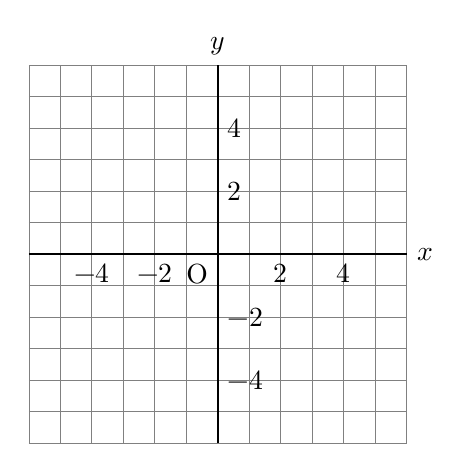
\begin{tikzpicture}[scale=0.4]
\draw[help lines] (-6,-6) grid (6,6);
\draw[thick](-6,0) -- (6,0)node[right]{$x$};
\draw[thick](0,-6) -- (0,6)node[above]{$y$};
\draw(0,0) node[below left]{O};
\foreach \x in {-4, -2, 2, 4} \draw ({\x},0) node[below]{$\x$};
\foreach \y in {-4, -2, 2, 4} \draw (0,{\y}) node[right]{$\y$};
\end{tikzpicture}

\end{multicols}

$y$が$x$の\framebox[1.5cm][c]{\raise 0.2ex\hbox{\textcircled{\scriptsize{ウ}}}}で、\ruby[g]{次}{つぎ}のような\ruby[g]{式}{しき}で\ruby[g]{表}{あらわ}されるとき、$y$は$x$に\framebox[1.5cm][c]{\raise 0.2ex\hbox{\textcircled{\scriptsize{ク}}}}するという。

$$
y = ax
$$

\ruby[g]{一定}{いってい}の\ruby[g]{数}{すう}やそれを\ruby[g]{表}{あらわ}す\ruby[g]{文字}{もじ}を\ruby[g]{定数}{ていすう}といい、\ruby[g]{上}{うえ}の\ruby[g]{式}{しき}のなかの\ruby[g]{文字}{もじ}$a$は\ruby[g]{定数}{ていすう}であり、\framebox[1.5cm][c]{\raise 0.2ex\hbox{\textcircled{\scriptsize{ケ}}}}という。$y$が$x$に\framebox[1.5cm][c]{\raise 0.2ex\hbox{\textcircled{\scriptsize{ク}}}}し、$x \neq 0$のとき、$\dfrac{y}{x}$の\ruby[g]{値}{あたい}は\ruby[g]{一定}{いってい}で、\framebox[1.5cm][c]{\raise 0.2ex\hbox{\textcircled{\scriptsize{ケ}}}}に\ruby[g]{等}{ひと}しい。

\framebox[1.5cm][c]{\raise 0.2ex\hbox{\textcircled{\scriptsize{ク}}}}のグラフは\ruby[g]{原点}{げんてん}を\ruby[g]{通}{とお}る\framebox[1.5cm][c]{\raise 0.2ex\hbox{\textcircled{\scriptsize{コ}}}}となる。

また、$y$が$x$の\framebox[1.5cm][c]{\raise 0.2ex\hbox{\textcircled{\scriptsize{ウ}}}}で、\ruby[g]{次}{つぎ}のような\ruby[g]{式}{しき}で\ruby[g]{表}{あらわ}されるとき、$y$は$x$に\framebox[1.5cm][c]{\raise 0.2ex\hbox{\textcircled{\scriptsize{サ}}}}するという。

$$
y = \dfrac{a}{x}
$$
\framebox[1.5cm][c]{\raise 0.2ex\hbox{\textcircled{\scriptsize{サ}}}}についても、\ruby[g]{定数}{ていすう}$a$を\framebox[1.5cm][c]{\raise 0.2ex\hbox{\textcircled{\scriptsize{ケ}}}}という。$y$が$x$に\framebox[1.5cm][c]{\raise 0.2ex\hbox{\textcircled{\scriptsize{サ}}}}するとき、$x$と$y$の\ruby[g]{積}{せき}$xy$は\ruby[g]{一定}{いってい}で、\framebox[1.5cm][c]{\raise 0.2ex\hbox{\textcircled{\scriptsize{ケ}}}}に\ruby[g]{等}{ひと}しい。

\framebox[1.5cm][c]{\raise 0.2ex\hbox{\textcircled{\scriptsize{サ}}}}のグラフはなめらかな2つの\ruby[g]{曲線}{きょくせん}になり、\framebox[1.5cm][c]{\raise 0.2ex\hbox{\textcircled{\scriptsize{シ}}}}とよばれる。このグラフは\ruby[g]{縦軸}{たてじく}、\ruby[g]{横軸}{よこじく}と\ruby[g]{交}{まじ}わらない。

\begin{itembox}[l]{語群}
\ruby[g]{係数}{けいすう}\hspace{1.5em}\ruby[g]{項}{こう}\hspace{1.5em}\ruby[g]{原点}{げんてん}\hspace{1.5em}\ruby[g]{比例}{ひれい}\hspace{1.5em}\ruby[g]{凡例}{はんれい}\hspace{1.5em}\ruby[g]{変数}{へんすう}\hspace{1.5em}\ruby[g]{定数}{ていすう}\hspace{1.5em}\ruby[g]{反比例}{はんぴれい}\hspace{1.5em}\ruby[g]{関数}{かんすう}\hspace{1.5em}\ruby[g]{間数}{かんすう}\hspace{1.5em}$v$\ruby[g]{軸}{じく}\hspace{1.5em}$x$\ruby[g]{軸}{じく}\hspace{1.5em}$y$\ruby[g]{軸}{じく}\hspace{1.5em} $z$\ruby[g]{軸}{じく}\hspace{1.5em}\ruby[g]{変域}{へんいき}\hspace{1.5em}\ruby[g]{凡例定数}{はんれいていすう}\hspace{1.5em}\ruby[g]{比例定数}{ひれいていすう}\hspace{1.5em}\ruby[g]{曲線}{きょくせん}\hspace{1.5em}\ruby[g]{半直線}{はんちょくせん}\hspace{1.5em}\ruby[g]{線分}{せんぶん}\hspace{1.5em}\ruby[g]{直線}{ちょくせん}\hspace{1.5em}\ruby[g]{二曲線}{にきょくせん}\hspace{1.5em}\ruby[g]{双曲線}{そうきょくせん}\hspace{1.5em}\ruby[g]{縦軸}{たてじく}\hspace{1.5em}\ruby[g]{横軸}{よこじく}\hspace{1.5em}\ruby[g]{絶対値}{ぜったいち}\hspace{1.5em}\ruby[g]{座標軸}{ざひょうじく}
\end{itembox}



\newpage

\noindent\fbox{\large\makebox[1em]{\text{\refstepcounter{kaunta}%
\arabic{kaunta}}}} \hspace{1pt}\ruby[g]{次}{つぎ}のような$x$と$y$の\ruby[g]{関係}{かんけい}について、$y$は$x$の\ruby[g]{関数}{かんすう}であるものを\ruby[g]{選}{えら}びなさい。

%
\begin{flushright}%
\footnotesize{<知・技2点>}%
\end{flushright}%


ア\hspace{1em} $x$\ruby[g]{歳}{さい}の\ruby[g]{人}{ひと}の\ruby[g]{体重}{たいじゅう}は$y\si{kg}$である。

イ\hspace{1em} \ruby[g]{半径}{はんけい}が$x \si{cm}$の\ruby[g]{円}{えん}の\ruby[g]{面積}{めんせき}を$y \si{cm}^2$とする。

ウ\hspace{1em} \ruby[g]{縦}{たて}の\ruby[g]{長}{なが}さが$x \si{cm}$の\ruby[g]{長方形}{ちょうほうけい}の\ruby[g]{面積}{めんせき}を$y \si{cm}^2$とする。

\vfill

\noindent\fbox{\large\makebox[1em]{\text{\refstepcounter{kaunta}%
\arabic{kaunta}}}} \hspace{1pt}\ruby[g]{変数}{へんすう}$x$が\ruby[g]{次}{つぎ}の\ruby[g]{値}{あたい}の\ruby[g]{範囲}{はんい}をとるとき、$x$の\ruby[g]{変域}{へんいき}を\ruby[g]{不等号}{ふとうごう}を\ruby[g]{使}{つか}って\ruby[g]{表}{あらわ}しなさい。

%
\begin{flushright}%
\footnotesize{<知・技$2\times 4$点>}%
\end{flushright}%


(\text{\refstepcounter{skaunta}%
\arabic{skaunta}})\hspace{2.5pt}1より\ruby[g]{大}{おお}きく、4\ruby[g]{以下}{いか}

(\text{\refstepcounter{skaunta}%
\arabic{skaunta}})\hspace{2.5pt}2\ruby[g]{未満}{みまん}

(\text{\refstepcounter{skaunta}%
\arabic{skaunta}})\hspace{2.5pt}$-3$より\ruby[g]{大}{おお}きい

(\text{\refstepcounter{skaunta}%
\arabic{skaunta}})\hspace{2.5pt}$-1$\ruby[g]{以上}{いじょう}$3$\ruby[g]{以下}{いか}

\setcounter{skaunta}{0}

\vfill

\begin{multicols}{2}
\noindent\fbox{\large\makebox[1em]{\text{\refstepcounter{kaunta}%
\arabic{kaunta}}}} \hspace{1pt}\ruby[g]{右}{みぎ}の\ruby[g]{図}{ず}で、\ruby[g]{点}{てん}A, B, C, Dの\ruby[g]{座標}{ざひょう}を\ruby[g]{答}{こた}えなさい。また、\ruby[g]{次}{つぎ}の\ruby[g]{点}{てん}E, F, Gを\ruby[g]{解答欄}{かいとうらん}に\ruby[g]{示}{しめ}しなさい。

%
\begin{flushright}%
\footnotesize{<知・技$2\times 7$点>}%
\end{flushright}%


E$(5, \, 4)$ 

F$(3, \, 0)$

G$(-3, \, 2)$

\columnbreak

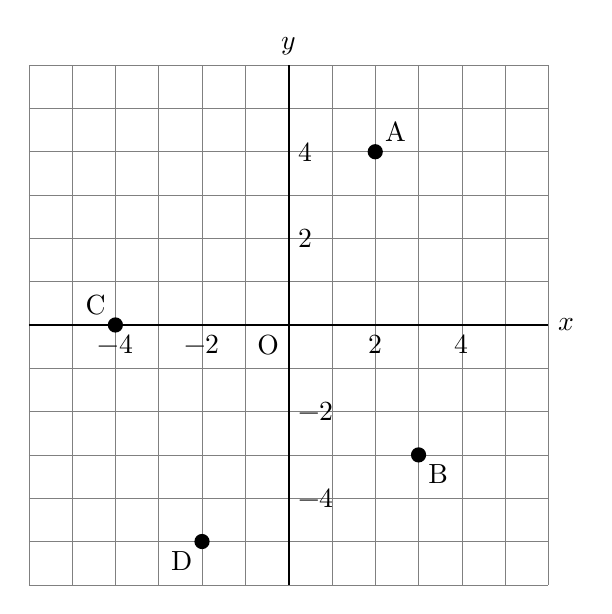
\begin{tikzpicture}[scale=0.55]
\draw[help lines] (-6,-6) grid (6,6);
\draw[thick](-6,0) -- (6,0)node[right]{$x$};
\draw[thick](0,-6) -- (0,6)node[above]{$y$};
\draw (0,0) node[below left]{O};
\foreach \x in {-4, -2, 2, 4} \draw ({\x},0) node[below]{$\x$};
\foreach \y in {-4, -2, 2, 4} \draw (0,{\y}) node[right]{$\y$};
\fill (2, 4) circle[radius=5pt] node[above right]{A};
\fill (3, -3) circle[radius=5pt] node[below right]{B};
\fill (-4, 0) circle[radius=5pt] node[above left]{C};
\fill (-2, -5) circle[radius=5pt] node[below left]{D};
\end{tikzpicture}

\end{multicols}

\vfill

\newpage

\noindent\fbox{\large\makebox[1em]{\text{\refstepcounter{kaunta}%
\arabic{kaunta}}}} \hspace{1pt}\ruby[g]{次}{つぎ}のア〜ウについて、$y$が$x$に\ruby[g]{比例}{ひれい}するものと、\ruby[g]{反比例}{はんぴれい}するものを\ruby[g]{選}{えら}び、\ruby[g]{記号}{きごう}で\ruby[g]{答}{こた}えなさい。また、\ruby[g]{式}{しき}も\ruby[g]{答}{こた}えなさい。

%
\begin{flushright}%
\footnotesize{<知・技6点>}%
\end{flushright}%


ア\hspace{1em}100kmの\ruby[g]{道}{みち}のりを\ruby[g]{時速}{じそく}$x$kmで\ruby[g]{走}{はし}ると、$y$\ruby[g]{時間}{じかん}かかる。

イ\hspace{1em}200ページの\ruby[g]{本}{ほん}を$x$ページ\ruby[g]{読}{よ}んだときの\ruby[g]{残}{のこ}りのページ\ruby[g]{数}{すう}は$y$ページである。

ウ\hspace{1em}\ruby[g]{底辺}{ていへん}が4cm、\ruby[g]{高}{たか}さが$x$cmの\ruby[g]{三角形}{さんかくけい}の\ruby[g]{面積}{めんせき}は$y$$\si{cm}^2$である。

\vfill

\noindent\fbox{\large\makebox[1em]{\text{\refstepcounter{kaunta}%
\arabic{kaunta}}}} \hspace{1pt}$y$は$x$に\ruby[g]{比例}{ひれい}し、$x = 3$のとき、$y = -9$です。このとき、\ruby[g]{次}{つぎ}の\ruby[g]{問}{とい}に\ruby[g]{答}{こた}えなさい。

%
\begin{flushright}%
\footnotesize{<知・技(1),(3),(4)2点、(2)4点>}%
\end{flushright}%


(\text{\refstepcounter{skaunta}%
\arabic{skaunta}})\hspace{2.5pt}$y$を$x$の\ruby[g]{式}{しき}で\ruby[g]{表}{あらわ}しなさい。

(\text{\refstepcounter{skaunta}%
\arabic{skaunta}})\hspace{2.5pt}\ruby[g]{次}{つぎ}の\ruby[g]{表}{ひょう}を\ruby[g]{完成}{かんせい}させなさい。
\begin{center}
\begin{tabular}{c|ccccccc}
\hline
$x$ & $\cdots$ & $-4$ & $0$ & $4$ & $\cdots$ & $12$ & $\cdots$ \\
\hline
$y$ & $\cdots$ &  &  &  & $\cdots$ & & $\cdots$ \\
\hline
\end{tabular}
\end{center}


(\text{\refstepcounter{skaunta}%
\arabic{skaunta}})\hspace{2.5pt}$x = 2$のときの$y$の\ruby[g]{値}{あたい}を\ruby[g]{求}{もと}めなさい。

(\text{\refstepcounter{skaunta}%
\arabic{skaunta}})\hspace{2.5pt}$x$の\ruby[g]{値}{あたい}が\ruby[g]{増加}{ぞうか}すると、$y$の\ruby[g]{値}{あたい}は\ruby[g]{増加}{ぞうか}しますか、それとも\ruby[g]{減少}{げんしょう}しますか。

\setcounter{skaunta}{0}

\vfill

\noindent\fbox{\large\makebox[1em]{\text{\refstepcounter{kaunta}%
\arabic{kaunta}}}} \hspace{1pt}$y$は$x$に\ruby[g]{反比例}{はんぴれい}し、$x = 4$のとき、$y = 6$です。このとき、\ruby[g]{次}{つぎ}の\ruby[g]{問}{とい}に\ruby[g]{答}{こた}えなさい。

%
\begin{flushright}%
\footnotesize{<知・技(1),(3),(4)2点、(2)4点>}%
\end{flushright}%


(\text{\refstepcounter{skaunta}%
\arabic{skaunta}})\hspace{2.5pt}$y$を$x$の\ruby[g]{式}{しき}で\ruby[g]{表}{あらわ}しなさい。

(\text{\refstepcounter{skaunta}%
\arabic{skaunta}})\hspace{2.5pt}\ruby[g]{次}{つぎ}の\ruby[g]{表}{ひょう}を\ruby[g]{完成}{かんせい}させなさい。

\begin{center}
\begin{tabular}{c|ccccccc}
\hline
$x$ & $\cdots$ & $-4$ & $0$ & $4$ & $\cdots$ & $12$ & $\cdots$ \\
\hline
$y$ & $\cdots$ &  & $\times$ &  & $\cdots$ & & $\cdots$ \\
\hline
\end{tabular}
\end{center}

(\text{\refstepcounter{skaunta}%
\arabic{skaunta}})\hspace{2.5pt}$x = -3$のときの$y$の\ruby[g]{値}{あたい}を\ruby[g]{求}{もと}めなさい。

(\text{\refstepcounter{skaunta}%
\arabic{skaunta}})\hspace{2.5pt}$x$の\ruby[g]{変域}{へんいき}が\ruby[g]{正}{せい}のとき、$x$の\ruby[g]{値}{あたい}が\ruby[g]{増加}{ぞうか}すると、$y$の\ruby[g]{値}{あたい}は\ruby[g]{増加}{ぞうか}しますか、それとも\ruby[g]{減少}{げんしょう}しますか。

\vfill

\newpage

\setcounter{skaunta}{0}
\begin{multicols}{2}
\noindent\fbox{\large\makebox[1em]{\text{\refstepcounter{kaunta}%
\arabic{kaunta}}}} \hspace{1pt}\ruby[g]{次}{つぎ}の\ruby[g]{問}{とい}に\ruby[g]{答}{こた}えなさい。

%
\begin{flushright}%
\footnotesize{<知・技(1)2点、(2),(3)4点>}%
\end{flushright}%


(\text{\refstepcounter{skaunta}%
\arabic{skaunta}})\hspace{2.5pt}\ruby[g]{右}{みぎ}の\ruby[g]{図}{ず}の\ruby[g]{点}{てん}Aの\ruby[g]{座標}{ざひょう}を\ruby[g]{求}{もと}めなさい。

(\text{\refstepcounter{skaunta}%
\arabic{skaunta}})\hspace{2.5pt}$y = 2x$のグラフをかきなさい。

(\text{\refstepcounter{skaunta}%
\arabic{skaunta}})\hspace{2.5pt}グラフが\ruby[g]{右}{みぎ}の\ruby[g]{図}{ず}の\ruby[g]{双曲線}{そうきょくせん}になる\ruby[g]{反比例}{はんぴれい}の\ruby[g]{式}{しき}を\ruby[g]{求}{もと}めなさい。

\columnbreak

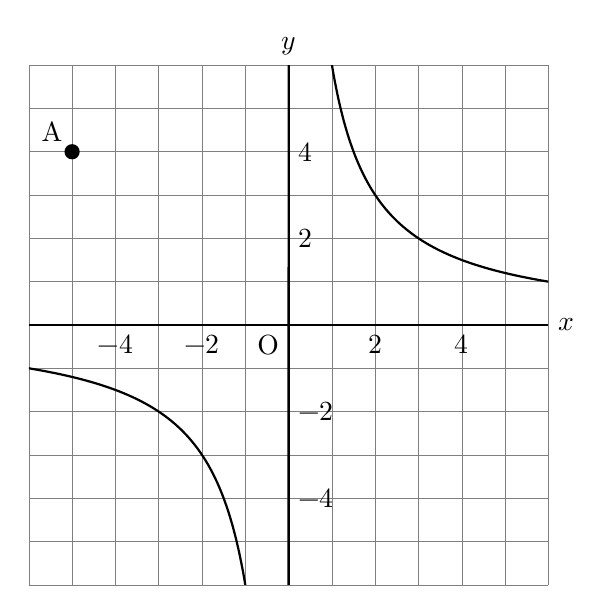
\begin{tikzpicture}[scale=0.55]
\draw[help lines] (-6,-6) grid (6,6);
\draw[thick](-6,0) -- (6,0)node[right]{$x$};
\draw[thick](0,-6) -- (0,6)node[above]{$y$};
\draw(0,0) node[below left]{O};
\foreach \x in {-4, -2, 2, 4} \draw ({\x},0) node[below]{$\x$};
\foreach \y in {-4, -2, 2, 4} \draw (0,{\y}) node[right]{$\y$};
\fill (-5,4) circle[radius=5pt] node[above left]{A};
\begin{scope}\clip(-6,-6) rectangle (6,6);
\draw [samples=100, smooth, thick, domain=-6:6] plot(\x, {6/\x});
\end{scope}
\end{tikzpicture}

\end{multicols}

\vfill

\noindent\fbox{\large\makebox[1em]{\text{\refstepcounter{kaunta}%
\arabic{kaunta}}}} \hspace{1pt}\ruby[g]{同}{おな}じ\ruby[g]{種類}{しゅるい}のクリップがあります。クリップ\ruby[g]{全体}{ぜんたい}の\ruby[g]{重}{おも}さは$120\si{g}$でした。そのうち、12\ruby[g]{個}{こ}を\ruby[g]{取}{と}り\ruby[g]{出}{だ}してその\ruby[g]{重}{おも}さをはかったら$18\si{g}$ありました。クリップは\ruby[g]{全部}{ぜんぶ}で\ruby[g]{何個}{なんこ}ありますか。

%
\begin{flushright}%
\footnotesize{<知・技2点>}%
\end{flushright}%


\vfill

\newpage

\noindent\fbox{\large\makebox[1em]{\text{\refstepcounter{kaunta}%
\arabic{kaunta}}}} \hspace{1pt}ある\ruby[g]{車}{くるま}いすマラソンで、もっとも\ruby[g]{速}{はや}い\ruby[g]{選手}{せんしゅ}は\ruby[g]{分速}{ふんそく}$300\si{m}$、もっとも\ruby[g]{遅}{おそ}い\ruby[g]{選手}{せんしゅ}は\ruby[g]{分速}{ふんそく}$120\si{m}$で\ruby[g]{走}{はし}ります。\ruby[g]{下}{した}の\ruby[g]{図}{ず}は\ruby[g]{横軸}{よこじく}に\ruby[g]{時間}{じかん}、\ruby[g]{縦軸}{たてじく}に\ruby[g]{距離}{きょり}をとって、もっとも\ruby[g]{速}{はや}い\ruby[g]{選手}{せんしゅ}ともっとも\ruby[g]{遅}{おそ}い\ruby[g]{選手}{せんしゅ}の\ruby[g]{時間}{じかん}と\ruby[g]{進}{すす}んだ\ruby[g]{距離}{きょり}をグラフにしたものです。

スタートしてから$6\si{km}$の\ruby[g]{地点}{ちてん}で\ruby[g]{応援}{おうえん}するとき、\ruby[g]{先頭}{せんとう}の\ruby[g]{選手}{せんしゅ}が\ruby[g]{通過}{つうか}してから\ruby[g]{何分後}{なんふんご}に、\ruby[g]{最後}{さいご}の\ruby[g]{選手}{せんしゅ}が\ruby[g]{通過}{つうか}するでしょうか。また、なぜその\ruby[g]{答}{こた}えになったのかをグラフを\ruby[g]{使}{つか}って\ruby[g]{説明}{せつめい}しなさい。ただし、\ruby[g]{選手}{せんしゅ}は\ruby[g]{一定}{いってい}の\ruby[g]{速}{はや}さで\ruby[g]{進}{すす}むものとする。

%
\begin{flushright}%
\footnotesize{<知・技6点>}%
\end{flushright}%


\begin{center}
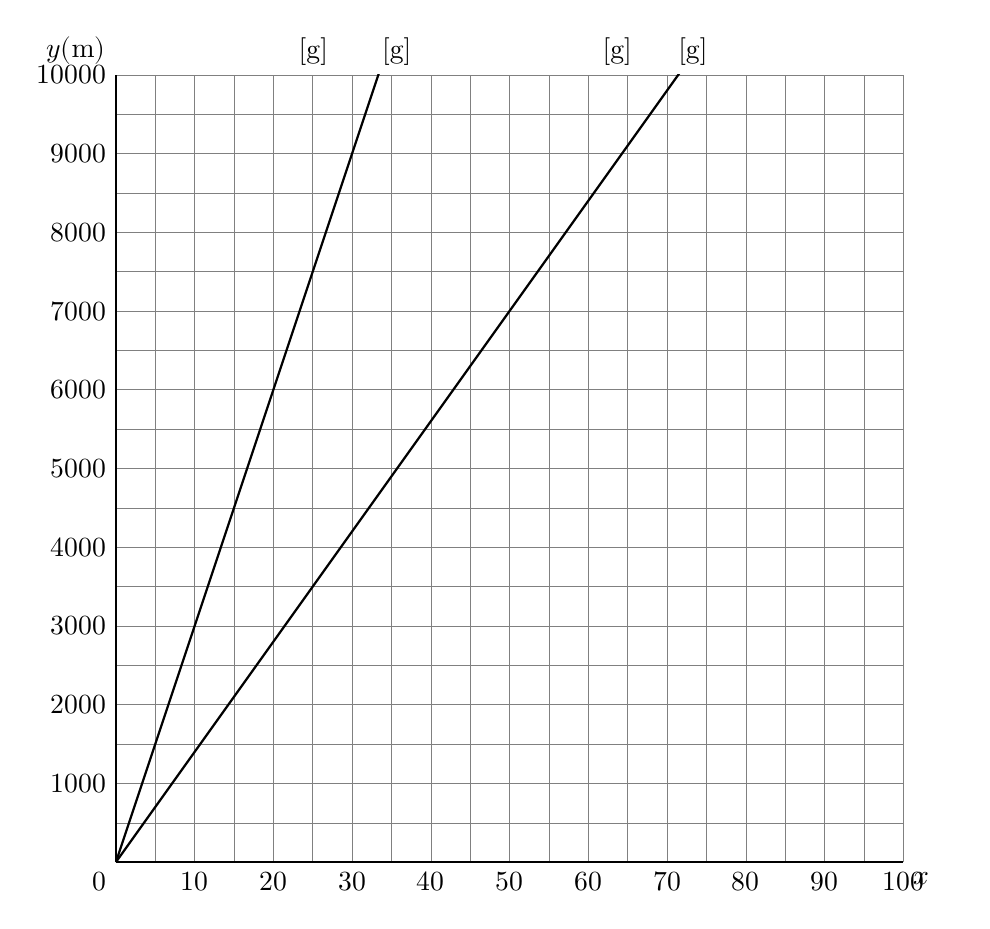
\begin{tikzpicture}[scale=0.5]
\draw[help lines] (0,0) grid (20,20);
\draw[thick](0,0) -- (20,0)node[below right]{$x\mbox{(分)}$};
\draw[thick](0,0) -- (0,20)node[above left]{$y(\si{m})$};
\draw(0,0) node[below left]{$0$};
\foreach \x in {1, 2, ..., 10} \draw ({2*\x},0) node[below]{$\x 0$};
\foreach \y in {1, 2, ..., 10} \draw (0,{2*\y}) node[left]{$\y 000$};
\draw ({20/3},20) node[above]{\ruby[g]{先頭}{せんとう}の\ruby[g]{選手}{せんしゅ}};
\draw ({100/7},20) node[above]{\ruby[g]{最後}{さいご}の\ruby[g]{選手}{せんしゅ}};
\begin{scope}\clip(0,0) rectangle (20,20);
\draw[thick, domain=0:20] plot(\x, {3*\x});
\draw[thick, domain=0:20] plot(\x, {7*\x/5});
\end{scope}
\end{tikzpicture}

\end{center}

\setcounter{skaunta}{0}

\newpage

\noindent\fbox{\large\makebox[1em]{\text{\refstepcounter{kaunta}%
\arabic{kaunta}}}} \hspace{1pt}\ruby[g]{科学}{かがく}クラブでは、\ruby[g]{文化祭}{ぶんかさい}でスライム\ruby[g]{作}{つく}りのイベントを\ruby[g]{行}{おこな}います。

%
\begin{flushright}%
\footnotesize{<思・判・表(1)3点、(2)5点>}%
\end{flushright}%


\begin{framed}
【スライムの\ruby[g]{作}{づく}り\ruby[g]{方}{かた}1\ruby[g]{人分}{りぶん}の\ruby[g]{材料}{ざいりょう}】

$\raise 0.2ex\hbox{\textcircled{\scriptsize{1}}}$\hspace{1em}\ruby[g]{大}{おお}きめの\ruby[g]{容器}{ようき}に、ぬるま\ruby[g]{湯}{ゆ}$100\si{ml}$とホウ\ruby[g]{砂}{さ}$4\si{g}$を\ruby[g]{入}{い}れてよくかき\ruby[g]{混}{ま}ぜる。

$\raise 0.2ex\hbox{\textcircled{\scriptsize{2}}}$\hspace{1em}$\raise 0.2ex\hbox{\textcircled{\scriptsize{1}}}$の\ruby[g]{容器}{ようき}に「のり」を$80\si{ml}$を\ruby[g]{加}{くわ}えて\ruby[g]{混}{ま}ぜる。

$\raise 0.2ex\hbox{\textcircled{\scriptsize{3}}}$\hspace{1em}$\raise 0.2ex\hbox{\textcircled{\scriptsize{2}}}$の\ruby[g]{液体}{えきたい}をかき\ruby[g]{混}{ま}ぜると、「のり」がだんだんとかたくなってくる。
\end{framed}

(\text{\refstepcounter{skaunta}%
\arabic{skaunta}})\hspace{2.5pt}\ruby[g]{必要}{ひつよう}な\ruby[g]{材料}{ざいりょう}を\ruby[g]{準備}{じゅんび}するとき、\ruby[g]{参加人数}{さんかにんずう}と\ruby[g]{必要}{ひつよう}な\ruby[g]{材料}{ざいりょう}の\ruby[g]{量}{りょう}について、「\ruby[g]{参加人数}{さんかにんずう}を\ruby[g]{決}{き}めると、それにともなって\ruby[g]{必要}{ひつよう}な\ruby[g]{材料}{ざいりょう}の\ruby[g]{量}{りょう}がただ1つ\ruby[g]{決}{き}まる」という\ruby[g]{関係}{かんけい}があります。

\hspace*{2em}\ruby[g]{下線部}{かせんぶ}を、\ruby[g]{次}{つぎ}のように\ruby[g]{表}{あらわ}すとき、\fbox{\phantom{あああ}}に\ruby[g]{当}{あ}てはまる\ruby[g]{言葉}{ことば}を\ruby[g]{書}{か}きなさい。

\begin{center}
\fbox{\phantom{材料の量}}は\fbox{\phantom{参加人数}}の\ruby[g]{関数}{かんすう}である。
\end{center}

\vfill

(\text{\refstepcounter{skaunta}%
\arabic{skaunta}})\hspace{2.5pt}30\ruby[g]{人分}{にんぶん}の\ruby[g]{材料}{ざいりょう}として、「のり」を$2400\si{ml}$\ruby[g]{用意}{ようい}しました。\ruby[g]{参加}{さんか}した\ruby[g]{人数}{にんずう}で「のり」を\ruby[g]{等分}{とうぶん}して\ruby[g]{使}{つか}い\ruby[g]{切}{き}るとき、1\ruby[g]{人分}{りぶん}の「のり」の\ruby[g]{量}{りょう}と、\ruby[g]{人数}{にんずう}は\ruby[g]{次}{つぎ}のような\ruby[g]{関係}{かんけい}になります。

\begin{center}
\begin{framed}
(1\ruby[g]{人分}{りぶん}の「のり」の\ruby[g]{量}{りょう})$=$ $2400 \div$(\ruby[g]{人数}{にんずう}) 
\end{framed}
\end{center}


\hspace*{1em} イベント\ruby[g]{当日}{とうじつ}、40\ruby[g]{人}{にん}が\ruby[g]{参加}{さんか}することになりました。\ruby[g]{人数}{にんずう}が$\dfrac{4}{3}$\ruby[g]{倍}{ばい}になっていることから、\ruby[g]{当日}{とうじつ}の1\ruby[g]{人分}{りぶん}の「のり」の\ruby[g]{量}{りょう}は、$80\si{ml}$を\ruby[g]{何倍}{なんばい}すればよいかを\ruby[g]{考}{かんが}えます。\ruby[g]{何倍}{なんばい}すればよいかを、\ruby[g]{次}{つぎ}のア、イの\ruby[g]{中}{なか}から1つ\ruby[g]{選}{えら}び、\ruby[g]{記号}{きごう}で\ruby[g]{答}{こた}えなさい。また、その\ruby[g]{理由}{りゆう}を\ruby[g]{下}{した}の\ruby[g]{言葉}{ことば}のうちどれかを\ruby[g]{使}{つか}って\ruby[g]{説明}{せつめい}しなさい。

\begin{center}
\begin{framed}
\hspace{3em} \ruby[g]{関数}{かんすう} \hspace{3em} \ruby[g]{比例}{ひれい} \hspace{3em} \ruby[g]{反比例}{はんぴれい} \hspace{3em}
\end{framed}
\end{center}

\hspace*{1em} ア \hspace{1em} 1\ruby[g]{人分}{りぶん}の「のり」の\ruby[g]{量}{りょう}を$\dfrac{4}{3}$\ruby[g]{倍}{ばい}にする。

\hspace*{1em} イ \hspace{1em} 1\ruby[g]{人分}{りぶん}の「のり」の\ruby[g]{量}{りょう}を$\dfrac{3}{4}$\ruby[g]{倍}{ばい}にする。

\vfill

\end{flushleft}

\end{document}
